\section{Deep Learning}

\begin{frame}[fragile]
  \frametitle{Introduction}
  \begin{itemize}
  \item What is Deep Learning?\\
  Deep Learning is a subfield of machine learning concerned with algorithms inspired by the structure and function of the brain called artificial neural networks.
  \item What is it used for?
  \begin{itemize}
  \item Self driving cars
  \item Beating humans in games
  \item Detecting spam in mails
  \item Forcasting stock prices
  \item Recognizing images in a picture
  \item Diagnosing illness (sometimes with better precision than doctors)
  \end{itemize}
  \end{itemize}
\end{frame}

\begin{frame}[fragile]
  \frametitle{University}
  Entry process for an university:
  \begin{itemize}
  \item Oral exam (x value)
  \item Written exam (y value)
  \end{itemize}
  Entry into the university is granted or denied based on x and y.\\
  \vspace{3mm}
  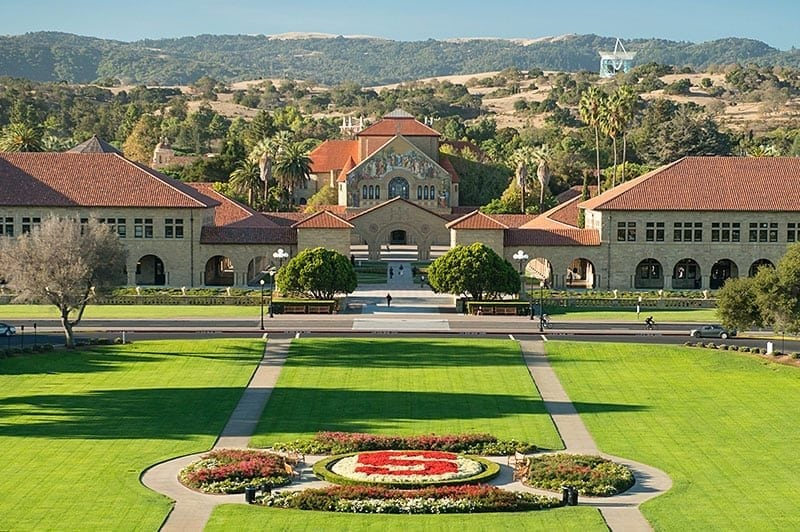
\includegraphics[scale=0.2]{img/stanford}
\end{frame}

\begin{frame}[fragile]
  \frametitle{University}
  Historical data: Green dots are accepted, red dots are rejected\\
  \vspace{3mm}
  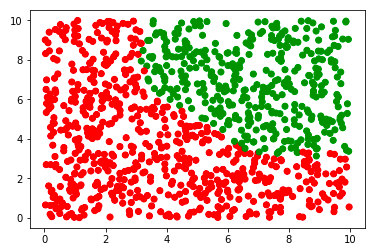
\includegraphics[scale=0.4]{img/uni_data}
\end{frame}

\begin{frame}[fragile]
  \frametitle{University}
  Deep Learning will now be used to find the line between the red and the green dots.
\end{frame}

\begin{frame}[fragile]
  \frametitle{University}
  To start with a easier example, we assume that the line is a straight line.
\end{frame}

\begin{frame}[fragile]
  \frametitle{University}
  To start with a easier example, we assume that the line is a straight line.
\end{frame}


